\documentclass{beamer}

\usetheme{PaloAlto}
\usepackage{pgfgantt}
\usepackage{eurosym}
\usepackage{listings}
\definecolor{azulUC3M}{RGB}{0,6,124}
\definecolor{rojoUC3M}{RGB}{186,50,50}
\definecolor{verdeUC3M}{RGB}{86,204,86}
\definecolor{white}{RGB}{255,255,255}
\definecolor{gray97}{gray}{.97}
\definecolor{gray90}{gray}{.90}
\definecolor{gray75}{gray}{.75}
\definecolor{gray45}{gray}{.45}
\lstset{ frame=Ltb,
     framerule=0pt,
     %aboveskip=0.5cm,
     framextopmargin=3pt,
     framexbottommargin=3pt,
     framexleftmargin=0.2cm,
     % xrightmargin=0.7cm,
     % xleftmargin=0.5cm,
     belowcaptionskip=0.5cm,
     framesep=0pt,
     rulesep=0.2pt,
     backgroundcolor=\color{gray97},
     rulesepcolor=\color{black},
     %
     stringstyle=\ttfamily,
     showstringspaces = false,
     basicstyle=\fontsize{7pt}{9pt}\ttfamily,
     commentstyle=\color{gray45},
     keywordstyle=\bfseries,
     %
     breaklines=true,
     literate= {<lambda>}{$\lambda$}1 {²}{{\textsuperscript{2}}}1 {µ}{$\upmu$}1
   }

   \lstdefinestyle{haskell}{
     language=Haskell,
   }

\usepackage[utf8]{inputenc}
\graphicspath{{../thesis/img/}}

%Information to be included in the title page:
\title[Agis: Search in Haskell]{Agis: Heuristic Search Library in Haskell}
\author[Diego Vicente]{Diego Vicente Martín \\
  {\small Supervisor: Carlos Linares López}}
\institute{Universidad Carlos III de Madrid}
\date{October 16th, 2017}

\logo{
\includegraphics[height=1.2cm]{slides-logo.png}}

\begin{document}

\frame{\titlepage}

\begin{frame}
  \frametitle{State of the Art}
  \begin{itemize}
  \item Heuristic search is a well-established discipline in Artificial
    Intelligence.
  \item Plenty of heuristic search frameworks exist in imperative languages.
  \item Few experiments in functional programming; only small pieces of code in
    Haskell.
  \end{itemize}
\end{frame}

\begin{frame}
  \frametitle{State of the Art}
  Haskell's main characteristics:
  \begin{itemize}
  \item Purely functional.
  \item Strong typing.
  \item Lazy evaluation.
  \item Concurrent abstractions.
  \end{itemize}
\end{frame}

\begin{frame}
  \frametitle{Motivation}
  Why?
  \begin{itemize}
  \item Concurrency/Parallelism is \textbf{hard}.
  \item Haskell provides a clean, minimal syntax.
  \item Functional programming is adequate for search.
  \item There is nothing like this already developed.
  \end{itemize}
\end{frame}

\begin{frame}
  \frametitle{Objectives}
  Develop a complete framework to work with heuristic search problems and
  research in Haskell, containing:
  \begin{itemize}
  \item A search algorithms library.
  \item Predefined search domains.
  \item Benchmark suites and tools.
  \item Full API documentation with examples.
  \end{itemize}
\end{frame}

\begin{frame}[fragile]
  \frametitle{Purity and $k$ Shortest Paths}
  \begin{itemize}
  \item It is not easy to translate typical pseudo-code to pure functional
    paradigm: no loops, no variables, no general state...
  \item Ideally, the output of functions should depend on its input only.
  \item This can be achieved by including a closed list per node.
  \item Inherently using infinite data structures let us solve the $k$ shortest
    paths problem as well as regular searches.
  \end{itemize}

\begin{lstlisting}[style=haskell]
sols = bfs problem  -- infinite list of solutions
print $ head sols   -- computes the first solution
print $ take 5 sols -- computes 5 first solutions
\end{lstlisting}
\end{frame}


\begin{frame}
  \frametitle{Use Cases}
  \begin{itemize}
  \item Solve a search problem.
  \item Get search statistics.
  \item Design a new search algorithm.
  \item Test a search algorithm.
  \item Benchmark a search algorithm.
  \end{itemize}
\end{frame}

\begin{frame}
  \frametitle{Project Artifacts}
  \begin{itemize}
  \item 28 functional requirements.
  \item 4 non-functional requirements.
  \item 2 \emph{type-signature graph} for visual intuition.
  \end{itemize}
\end{frame}

\begin{frame}
  \frametitle{Type-Signature Graphs}
  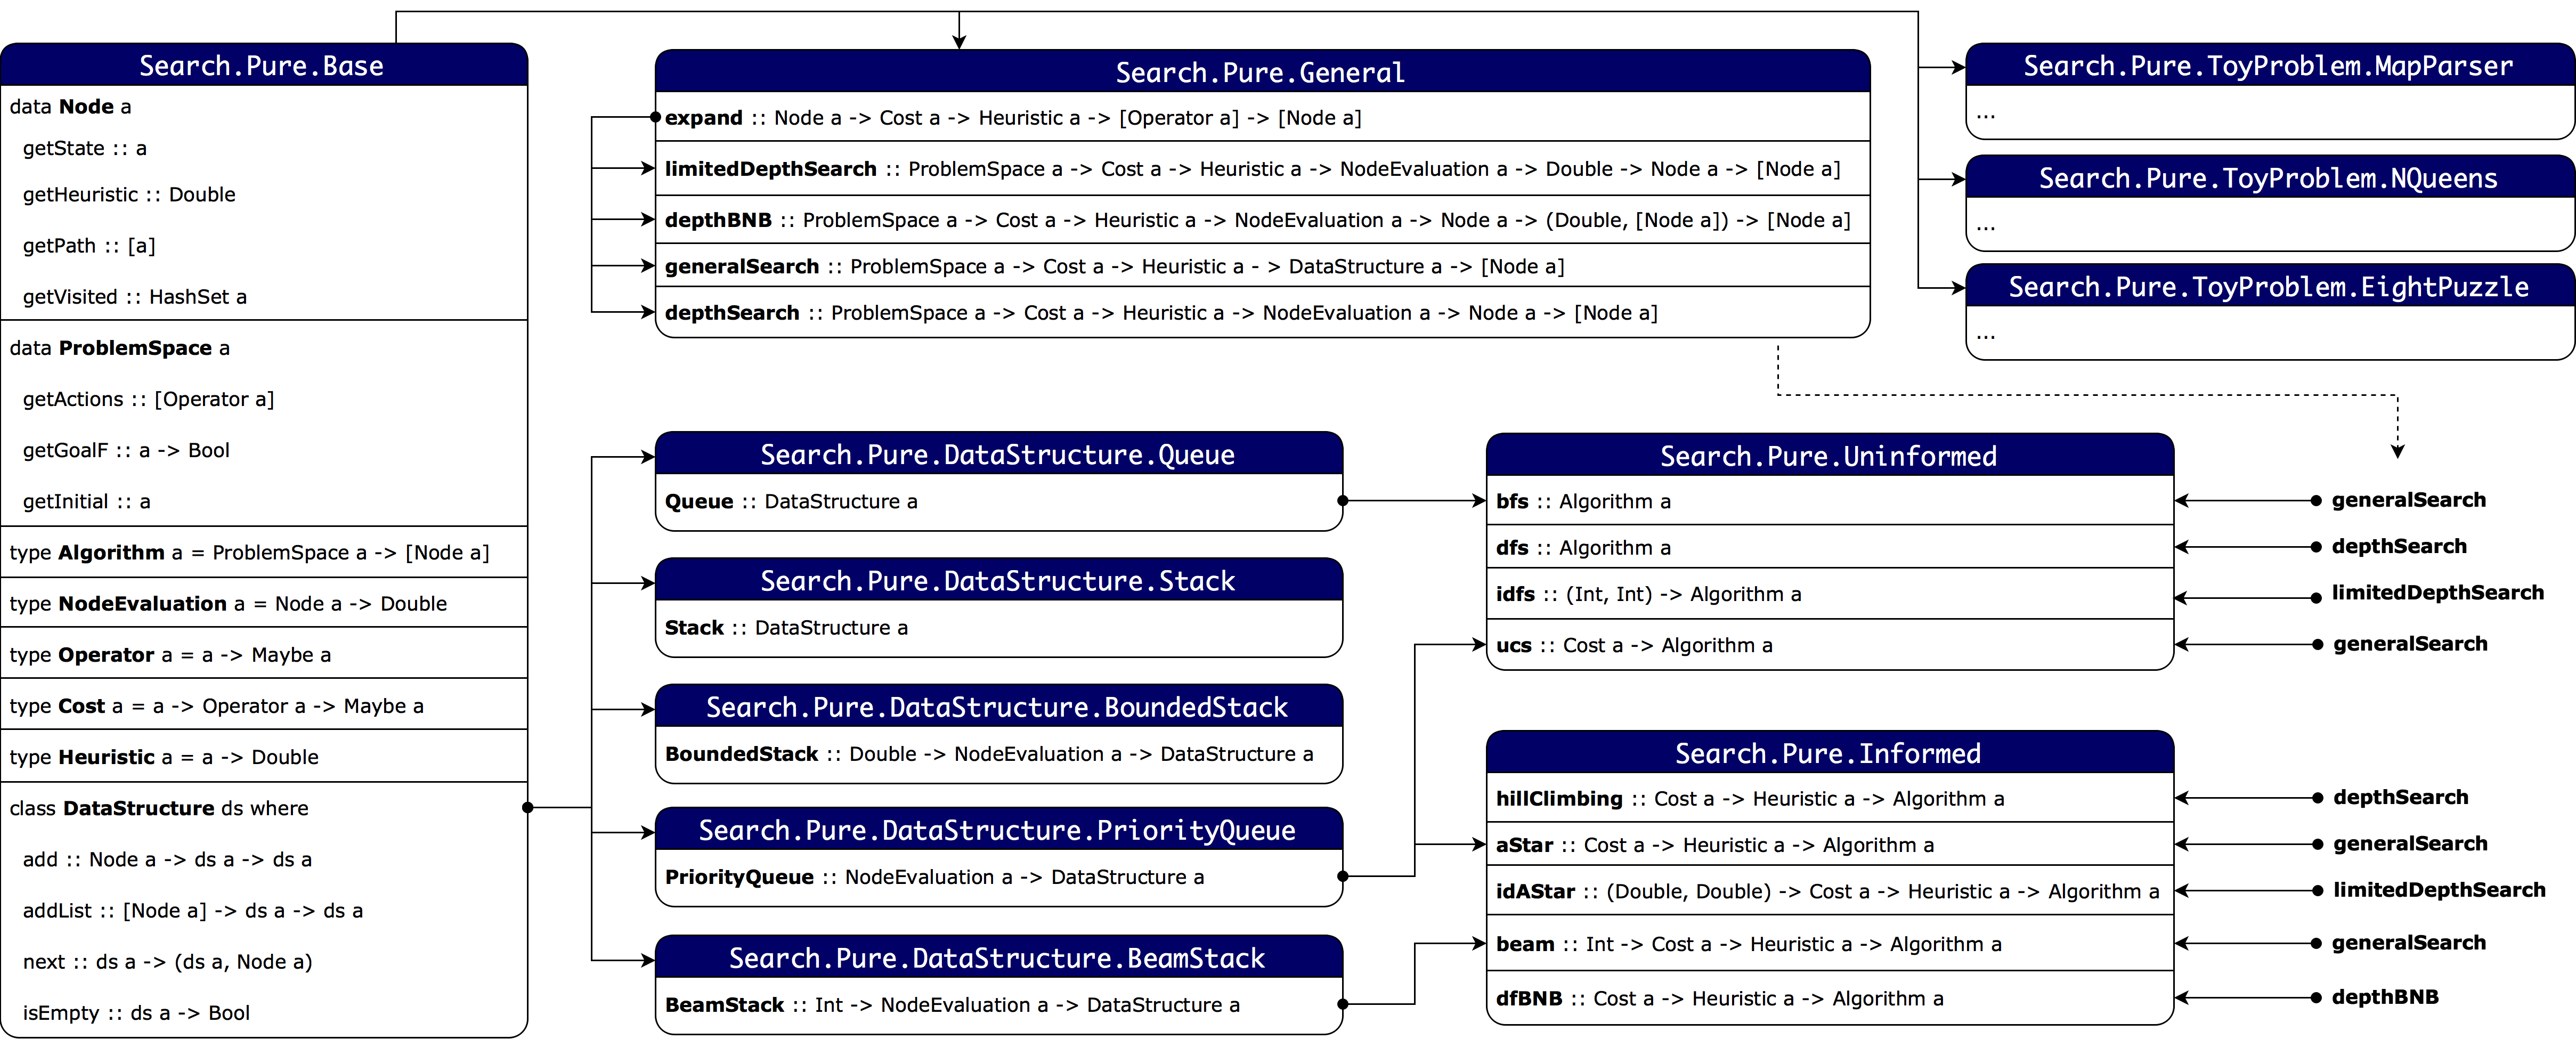
\includegraphics[width=\textwidth]{type-graph-pure.png}
\end{frame}

\begin{frame}
  \frametitle{General Search Implementation}
  A primitive general search is inspired in Russel and Norvig's
  \emph{Artificial Intelligence: A Modern Approach} algorithm
  \texttt{GENERAL\_SEARCH}:
  \begin{itemize}
  \item Uses a data structure to store expanded nodes.
  \item The algorithm's behavior is defined by the data structure.
  \end{itemize}
\end{frame}

\begin{frame}[fragile]
  \frametitle{General Search Implementation}
\begin{lstlisting}[style=haskell]
generalSearch :: (DataStructure ds, Eq a, Hashable a)
  => ProblemSpace a
  -- ^ 'ProblemSpace' to be solved
  -> Cost a
  -- ^ 'Cost' function to use
  -> Heuristic a
  -- ^ 'Heuristic' function to use
  -> ds a
  -- ^ 'DataStructure' that manages the node expansion
  -> [Node a]
  -- ^ Returns the list of all final nodes (solutions)

generalSearch problem g h nodes
  | isEmpty nodes = []
  | getGoalF problem (getState n) =
    n : generalSearch problem g h nodes'
  | otherwise = generalSearch problem g h ds'

  where (nodes', n) = next nodes
        expanded = expand n g h (getActions p)
        ds' = addList expanded nodes'
\end{lstlisting}
\end{frame}

\begin{frame}[fragile]
  \frametitle{Data Structures}
  To change the behavior of the \texttt{generalSearch} method, it is possible
  to use a \texttt{DataStructure} type.
  \begin{itemize}
  \item Implements the class defining the necessary methods.
  \item These methods should be enough to define most kinds of search
    behaviors.
  \item Some examples provided in the library included a queue, a stack or a
    priority queue.
  \end{itemize}
\begin{lstlisting}[style=haskell]
class DataStructure ds where

  add :: (Eq a, Hashable a) => Node a -> ds a -> ds a

  addList :: (Eq a, Hashable a) => [Node a] -> ds a -> ds a

  next :: (Eq a, Hashable a) => ds a -> (ds a, Node a)

  isEmpty :: (Eq a, Hashable a) => ds a -> Bool
\end{lstlisting}
\end{frame}


\begin{frame}
  \frametitle{Linear-Memory Search Implementation}
  Many algorithms require linear-memory cost to be valid primitives.
  \begin{itemize}
  \item Use \texttt{map} and recursion to expand the nodes.
  \item General depth-first behavior, can be changed by the functions passed to
    it.
  \item Use of \texttt{map} is cheap and enables high-level concurrent
    abstractions.
  \item Alternative version can receive a node evaluation function and a limit
    to perform bounded depth-first search.
  \end{itemize}
\end{frame}

\begin{frame}[fragile]
  \frametitle{Linear-Memory Implementation}
\begin{lstlisting}[style=haskell]
depthSearch :: (Eq a, Hashable a)
  => ProblemSpace a
  -- ^ 'ProblemSpace' to be solved
  -> Cost a
  -- ^ 'Cost' function to use
  -> Heuristic a
  -- ^ 'Heuristic' function to use
  -> NodeEvaluation a
  -- ^ 'NodeEvaluation' to sort the expanded nodes
  -> Node a
  -- ^ Current 'Node' to be expanded
  -> [Node a]
  -- ^ Returns the list of all solutions

depthSearch problem g h f node
  | getGoalF problem (getState node) = return node
  | otherwise = concatMap (depthSearch problem g h f) sorted
    where sorted = sortBy (\n n' -> compare (f n) (f n')) ns
          ns = expand node g h (getActions problem)
\end{lstlisting}
\end{frame}

\begin{frame}
  \frametitle{Branch and Bound Search Implementation}
  Another primitive to use is a general Branch and Bound search:
  \begin{itemize}
  \item Branch and Bound algorithms uses the best solution found cost as
    current bound; then keeps expanding the tree with new solutions.
  \item Use a \texttt{fold} to traverse the tree with the best solution and
    current bound until search space is exhausted.
  \item Does not find the best $k$ solutions.
  \end{itemize}
  \centering
  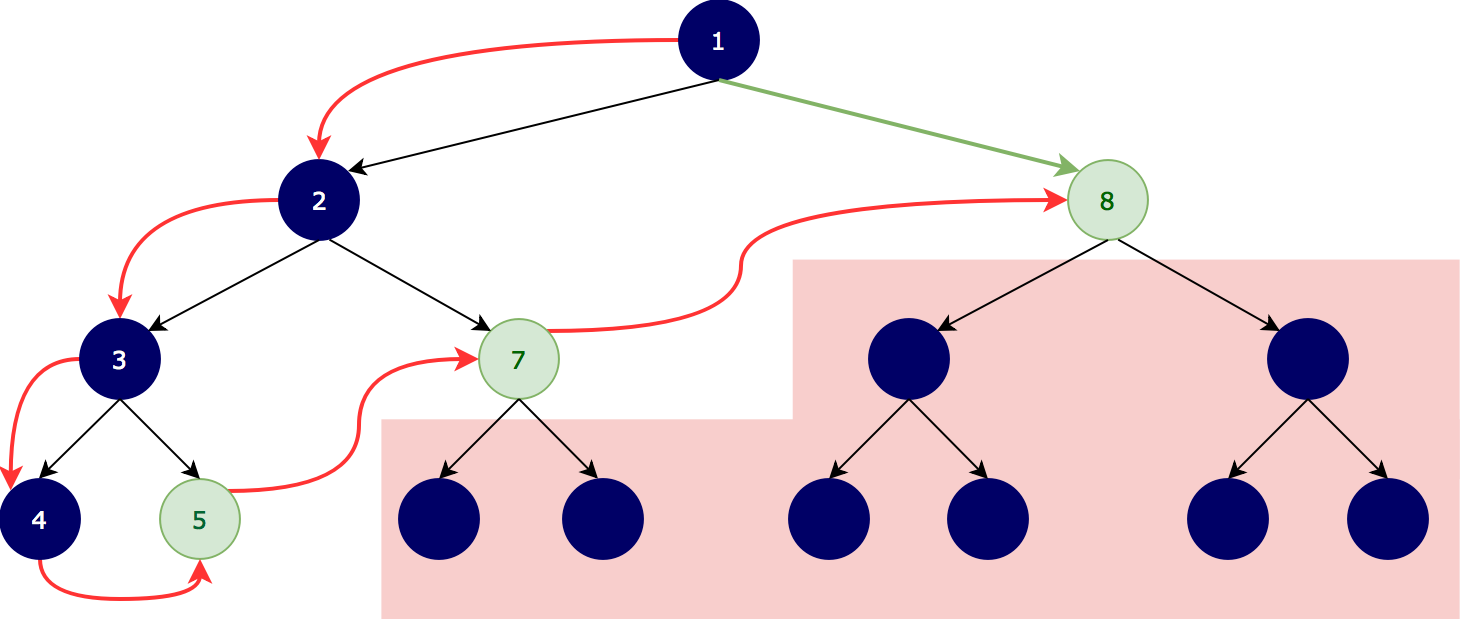
\includegraphics[width=0.7\textwidth]{dfbnb.png}
\end{frame}

\begin{frame}[fragile]
  \frametitle{Branch and Bound Implementation}
\begin{lstlisting}[style=haskell]
depthBNB :: (Eq a, Hashable a)
  => ProblemSpace a
  -- ^ 'ProblemSpace' to be solved
  -> Cost a
  -- ^ 'Cost' function to use
  -> Heuristic a
  -- ^ 'Heuristic' function to use
  -> NodeEvaluation a
  -- ^ 'NodeEvaluation' to sort and bound the expanded nodes
  -> Node a
  -- ^ Current 'Node' to be expanded
  -> (Double, [Node a])
  -- ^ The current bound and intermediate solutions found
  -> (Double, [Node a])
  -- ^ The final bound and all solutions found
depthBNB problem g h f n (l, sol) = foldl bnbStep (l, sol) sorted
  where sorted = sortBy (\n n' -> compare (f n) (f n')) expanded
        expanded = expand n g h (getActions problem)
        bnbStep (bound, solutions) n
          | f n >= bound = (bound, solutions)
          | getGoalF problem (getState n) = (f n, n:solutions)
          | otherwise = depthBNB problem g h f n (bound, solutions)
\end{lstlisting}
\end{frame}

\begin{frame}
  \frametitle{The Search Monad}
  \begin{itemize}
  \item It is not possible to obtain accurate statistics in recursive calls.
  \item No access to global state of the computer, and therefore context.
  \item Using a monad, we can encapsulate the context with the solution and
    define how to combine contexts together.
  \item If we define our structure as a monad, we can use \texttt{do} notation
    inside Haskell.
  \end{itemize}
\end{frame}

\begin{frame}[fragile]
  \frametitle{\texttt{do} Notation}
\begin{lstlisting}[style=haskell]
-- Unsweet version
greet :: IO String
greet = print "Name? " >>
          (getLine >>= (\name -> print $ "hello " ++ name))

-- Do notation as syntactic sugar
greet' :: IO String
greet' = do
  print "Name? "
  name <- getLine
  print $ "hello " ++ name
\end{lstlisting}
\end{frame}

\begin{frame}[fragile]
  \frametitle{The Search Monad}
  \begin{itemize}
  \item The monad (\texttt{SearchM}) will pack together a node with its context
    (a \texttt{Statistics} record), which contains:
    \begin{itemize}
    \item Number of nodes expanded.
    \item Number of nodes enqueued.
    \item Maximum length of the data structure.
    \end{itemize}
  \item The way to join to \texttt{Statistics} is defined to join contexts in
    recursive calls.
  \item \texttt{SearchM} has to implement the \texttt{Functor} and
    \texttt{Applicative} classes before the \texttt{Monad} class.
  \end{itemize}

  \begin{lstlisting}[style=haskell]
data SearchM a = SearchM { getNode  :: a
                         , getStats :: Statistics
                         }
\end{lstlisting}
\end{frame}

\begin{frame}[fragile,fragile]
  \frametitle{The Search Monad}
  \begin{itemize}
  \item All monads have to follow the three monad laws to prevent unexpected
    behavior in \texttt{do} notation:
    \begin{itemize}
    \item Left identity: $unit \  x \star f = f(x) $
    \item Right identity: $m \star \  \lambda x \rightarrow unit \  x = m$
    \item Associativity: $m \star f \star g = m \star (\lambda x \rightarrow
      f(x) \star g)$
    \end{itemize}
  \item The implementation has been formally proven to follow these laws using
    predicate logic.
  \end{itemize}

\begin{lstlisting}[style=haskell]
instance Monad SearchM where
  return = pure
  SearchM n s >>= f =
    let SearchM n' s' = f n
    in SearchM n' (mergeStats s s')
\end{lstlisting}
\end{frame}

\begin{frame}
  \frametitle{Disadvantages of the Search Monad}
  \begin{itemize}
  \item The statistics are computed for the whole search, which breaks lazy
    evaluation.
  \item A way to solve this is to use a classic behavior and return the first
    solution only.
  \item Therefore, the monadic version of the library does not solve the $k$
    shortest paths problem.
  \end{itemize}
\end{frame}

\begin{frame}[fragile]
  \frametitle{Example of Monadic Primitive}
\begin{lstlisting}[style=haskell]
generalSearch :: (DataStructure ds, Eq a, Hashable a)
  => ProblemSpace a
  -> Cost a
  -> Heuristic a
  -> ds a
  -> SearchM (Maybe (Node a))

generalSearch problem g h nodes
  | isEmpty nodes = do
      logExpanded
      return Nothing
  | getGoalF problem (getState n) = do
      logExpanded
      return (Just n)
  | otherwise = do
      logExpanded
      logEnqueued (length expanded)
      logLength ds'
      generalSearch problem g h ds'

  where (nodes', n) = next nodes
        expanded = expand n g h (getActions problem)
        ds' = addList expanded nodes'
\end{lstlisting}
\end{frame}

\begin{frame}
  \frametitle{Features}
  \begin{itemize}
  \item \emph{Uninformed algorithms}: Breadth-First Search, Depth-First Search,
    Iterative-Deepening Depth-First Search, Beam Search, Uniform Cost Search.
  \item \emph{Informed algorithms}: Hill-Climbing, A*, Iterative-Deepening A*,
    Depth-First Branch and Bound.
  \item \emph{Search domains}: 8-Puzzle, N-Queens, MovingAI Map Parser.
  \item Several \texttt{criterion} benchmarking suites provided for each of the
    search domains.
  \end{itemize}
\end{frame}

\begin{frame}
  \frametitle{Testing}
  A suite of unit and integration tests is included in library.
  \begin{itemize}
  \item The test suite reflects the structure of the modules 1:1 to ensure full
    coverage.
  \item These tests check all different branches for each function as well as
    each algorithm in each search domain (if applicable).
  \item The suite is formed by 156 successful examples.
  \end{itemize}
\end{frame}

\begin{frame}
  \frametitle{Benchmarking}
  Apart from the test, thorough benchmark is required to prove correctness of
  the algorithms.
  \begin{itemize}
  \item In general, memory/time/node expansion behave in every algorithm as
    expected.
  \item Results show that some algorithms are not suitable for certain
    problems.
  \item Remarkable outlier: \texttt{PriorityQueue}-based algorithms show
    strangely poor performance in problem with long queues.
  \end{itemize}
\end{frame}

\begin{frame}
  \frametitle{Searching the Leak}
  \begin{itemize}
  \item Using the \texttt{RTS+} is possible to generate a profile of the code.
  \item Using the \texttt{profiling} executable designed was possible to
    benchmark the code intensively.
  \item The problem was pinned to be associated to the space allocation
    performed by the \texttt{heap} package and the garbage collection of it.
  \end{itemize}
\end{frame}

\begin{frame}
  \frametitle{Searching for Solutions}
  \begin{itemize}
  \item Try to change the package used to a different one (\texttt{psqueues}).
  \item Try to search the implementation of the queue (using union or folds).
  \item Brute-force the garbage collector to understand its influence.
  \end{itemize}
  \centering
  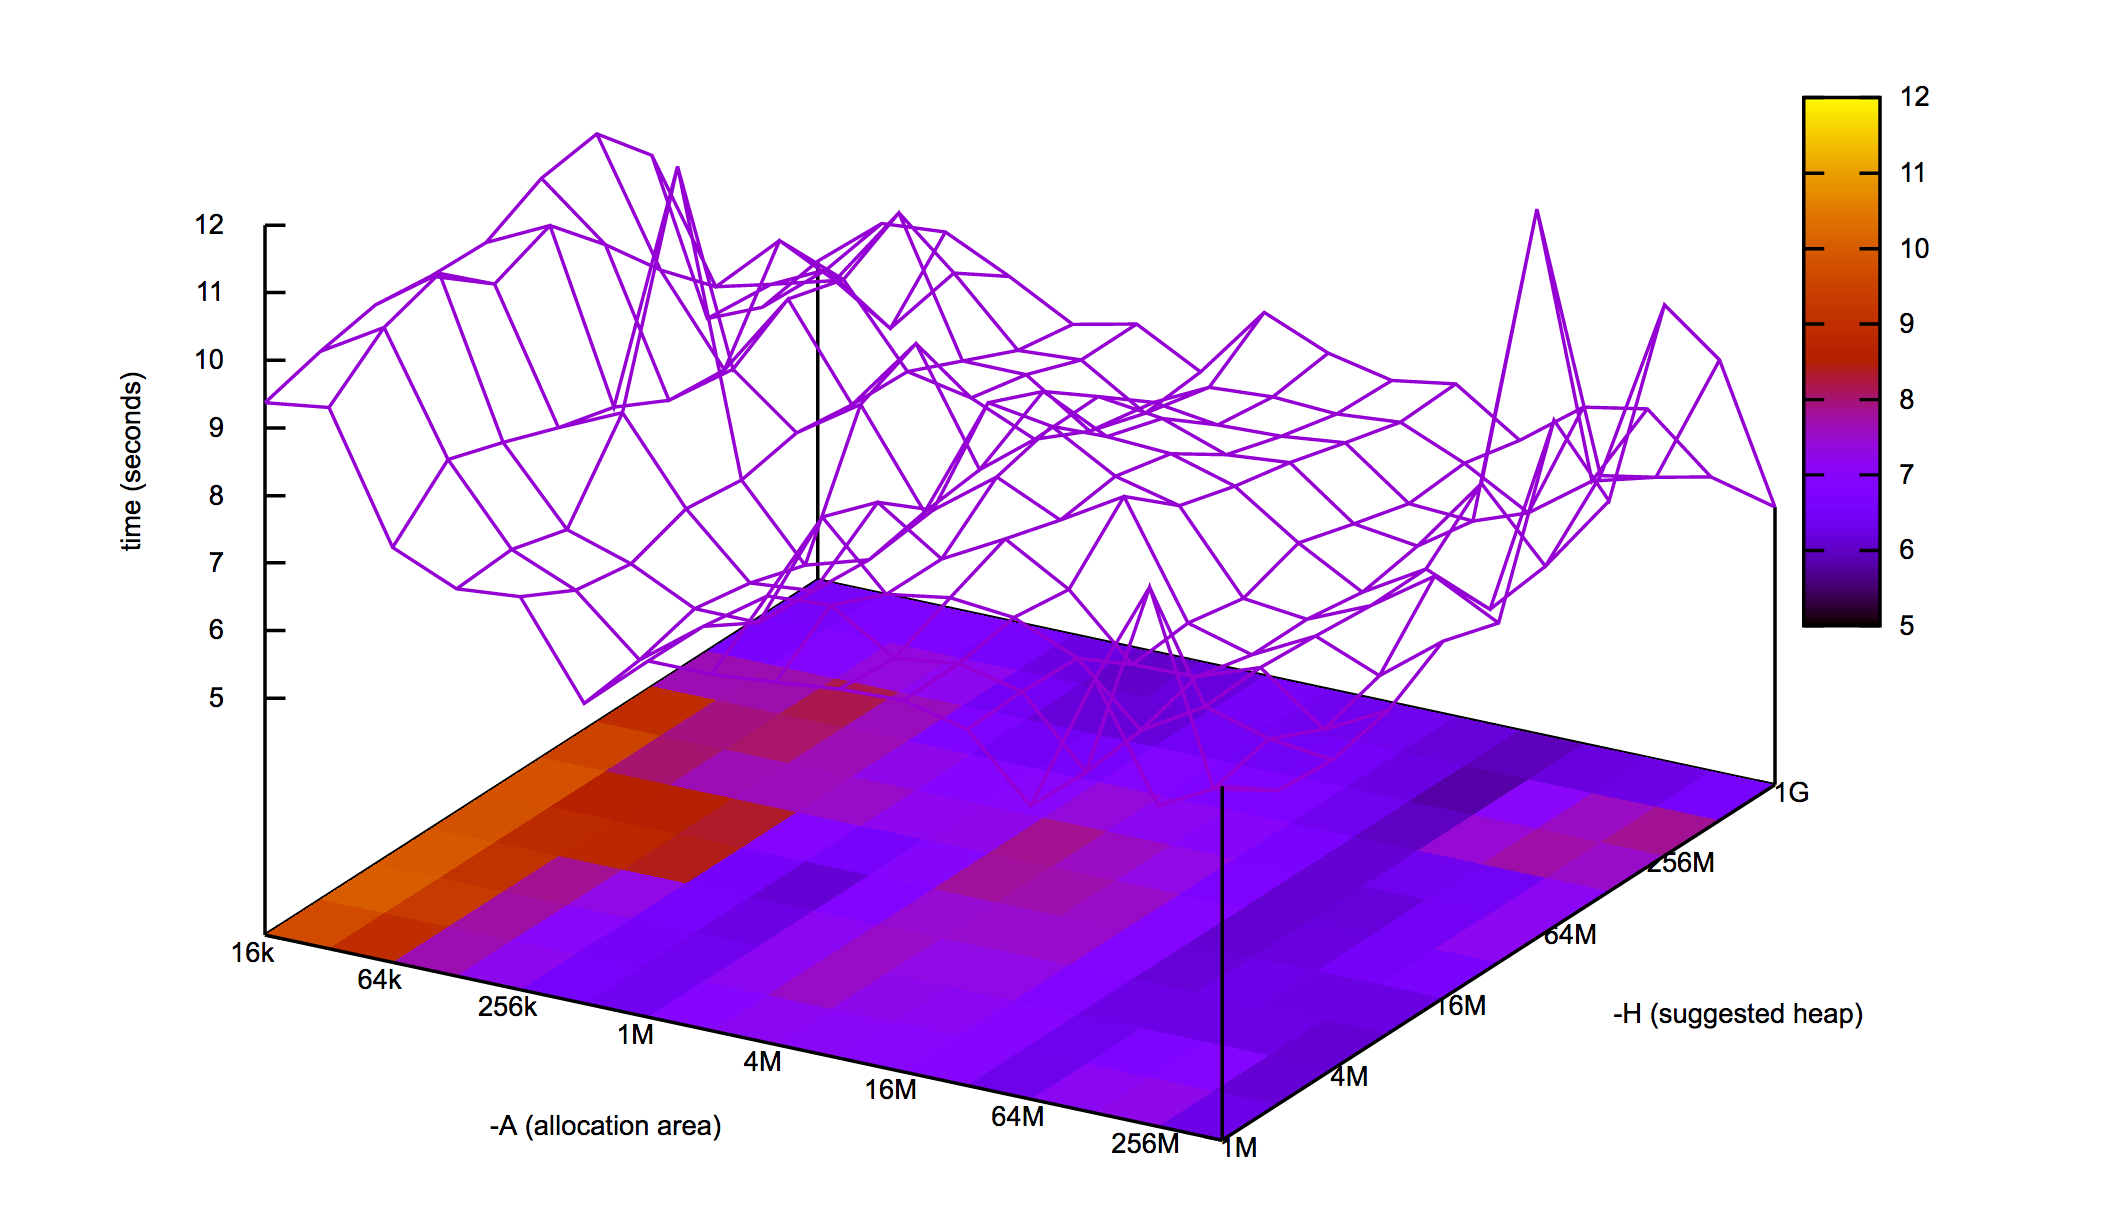
\includegraphics[width=0.7\textwidth]{gc-tuning.png}
\end{frame}

\begin{frame}
  \frametitle{Searching for Solutions}
  \begin{itemize}
  \item None of the previous options solved completely the problem.
  \item The definitive way to solve it would be to implement a mutable, $O(1)$
    extraction priority queue in Haskell.
  \item Out of the scope of the thesis.
  \end{itemize}
\end{frame}

\begin{frame}
  \frametitle{Organization}
  \begin{figure}[ht]
  \scalebox{.5}{
  \centering
  \begin{ganttchart}[vgrid = dotted, hgrid = dotted, compress calendar,
    time slot format=isodate-yearmonth, x unit = 8mm,
    group left shift = 0.1, group right shift = -0.1,
    title/.append style={fill=azulUC3M, draw=white, thick},
    title label font=\color{white}\ttfamily,
    title height = 1,
    group/.append style={fill=azulUC3M},
    group label font = \small,
    bar/.append style={fill=azulUC3M, draw=none, rounded corners=3pt},
    bar label font = \small,
    milestone/.append style={draw=azulUC3M, fill=azulUC3M},
    milestone label font = \small,
    link/.append style={azulUC3M}]
    {2016-09}{2017-09}
    \gantttitlecalendar{year, month} \\

    \ganttgroup{Phases}{2016-09}{2017-02}
    \ganttgroup{}{2017-03}{2017-06}
    \ganttgroup{}{2017-07}{2017-09} \\

    % \ganttgroup{Research}{2016-09}{2017-06} \\
    \ganttbar{Previous Research}{2016-09}{2016-10} \\
    \ganttlinkedbar{Analysis}{2016-10}{2016-11} \\
    \ganttlinkedbar{Design and Modelling}{2016-12}{2017-02} \\
    \ganttlinkedmilestone{Initial design}{2017-02} \\

    % \ganttgroup{Development}{2017-03}{2017-09} \\
    \ganttlinkedbar{Implementation}{2017-03}{2017-05} \\
    \ganttlinkedbar{Testing}{2017-04}{2017-06} \\
    \ganttlinkedmilestone{\texttt{v0.1.0.0}}{2017-06} \\

    % \ganttgroup{Testing}{2017-07}{2017-09} \\
    \ganttlinkedbar{Iteration}{2017-07}{2017-08} \\
    \ganttlinkedmilestone{\texttt{v0.2.0.0}}{2017-08}
  \end{ganttchart}
  }
\end{figure}
\end{frame}

\begin{frame}[fragile]
  \frametitle{Budget}

  A brief summary of the project's accounting:

  \begin{table}[!htbp]
    \centering
   \begin{tabular}{| l | r |}
     \hline
     Concept & Total \\
     \hline
     Personnel Costs & 7250 \euro \\
     Equipment Costs & 546.65 \euro \\
     Indirect Costs  & 779.97 \euro \\
     \hline
     Project Costs   & 8579.62 \euro \\
     Risk            & +10\% \\
     Benefits        & +10\% \\
     \hline
     \hline
     \textbf{Project Budget}  & \textbf{10295.54 \euro} \\
     \hline
   \end{tabular}
 \end{table}

\end{frame}

\begin{frame}
  \frametitle{Legal}
  The project is planned to be open-sourced in the near future:
  \begin{itemize}
  \item The only legal requirement to take into account is the license of the
    framework.
  \item The framework will be distributed as a Haskell package under the GNU
    General Public License v3.0.
  \item A contributor's workflow is defined along with the package repository.
  \end{itemize}
\end{frame}

\begin{frame}
  \frametitle{Socio-economic Impact}
  The project shows great potential:
  \begin{itemize}
  \item In education, where it provides a clean and easy syntax along with an
    interactive environment to work on search algorithms.
  \item In research, where fast iteration on algorithm design and comparison
    with existing baseline algorithms is crucial.
  \item If the project matures adequately, it can provide an easy way to work
    on search in an inherently concurrent environment.
  \end{itemize}
\end{frame}


\begin{frame}
  \frametitle{Conclusions and Future Work}
  Some conclusions drawn:
  \begin{itemize}
  \item It is possible to successfully implement search algorithms in a
    stateless environment.
  \item Purely functional programming restricts the implementation but offers a
    great deal of advantages.
  \item Heuristic search is an interesting topic to research in the functional
    programming paradigm.
  \end{itemize}

  Future work:
  \begin{itemize}
  \item Fix (or workaround) the \texttt{PriorityQueue} issue.
  \item New algorithms, data structures, search domains.
  \item Better automatization tools.
  \end{itemize}
\end{frame}

\begin{frame}
  \frametitle{Thank you!}
  \centering {\huge Questions?}
\end{frame}
\end{document}

%%% Local Variables:
%%% mode: latex
%%% TeX-master: t
%%% End:
